\chapter{System Implementation} \label{ch:implementation}
\section{Overview of Network Functions} \label{sec:desc_nfv_overview}

Our network functions (Fig. \ref{fig:desc_nfv_overview}) are designed with SDN-enabled NFV architecture concept \cite{sdn-enabled}, using the synergies between computer infrastructures (NFVs) and network infrastructures (NFVIs) \cite{etsi-nfv-terminology, etsi-nfv-infra}. An NFV is a VNF controller, mainly used for addressing stateful processing and NFVI is an SDN switch used for stateless processing.

\subsection{Stateful Processing Component}
This component is used to control the workflow, maintain the state associated with the VNF, and provide an interface for service providers or customers to configure and update the behavior of the stateless datapath processing component. We used an SDN controller to implement the VNF controller; and notably, we use southbound APIs of the SDN controller framework to manage the interface between the stateful and stateless components with the OpenFlow protocol, which was originally designed for this purpose.

\subsection{Stateless Processing Component}
Stateless processing component is implemented by SDN datapath resources and is optimized for data plane traffic processing. Because an SDN switch can be decoupled with control plane and data plane, the switch can accept the control messages from the stateful processing component.

By using the advantages of this architecture, we can assign stateless or light-weight state work to the SDN switch (e.g., packet filtering and packet counting) to reduce the load on the computing resources. If we want to update our service, we are required to update only the stateful component, because the stateless component merely follows the commands from the stateful component.

\begin{figure}[!t]
\centering
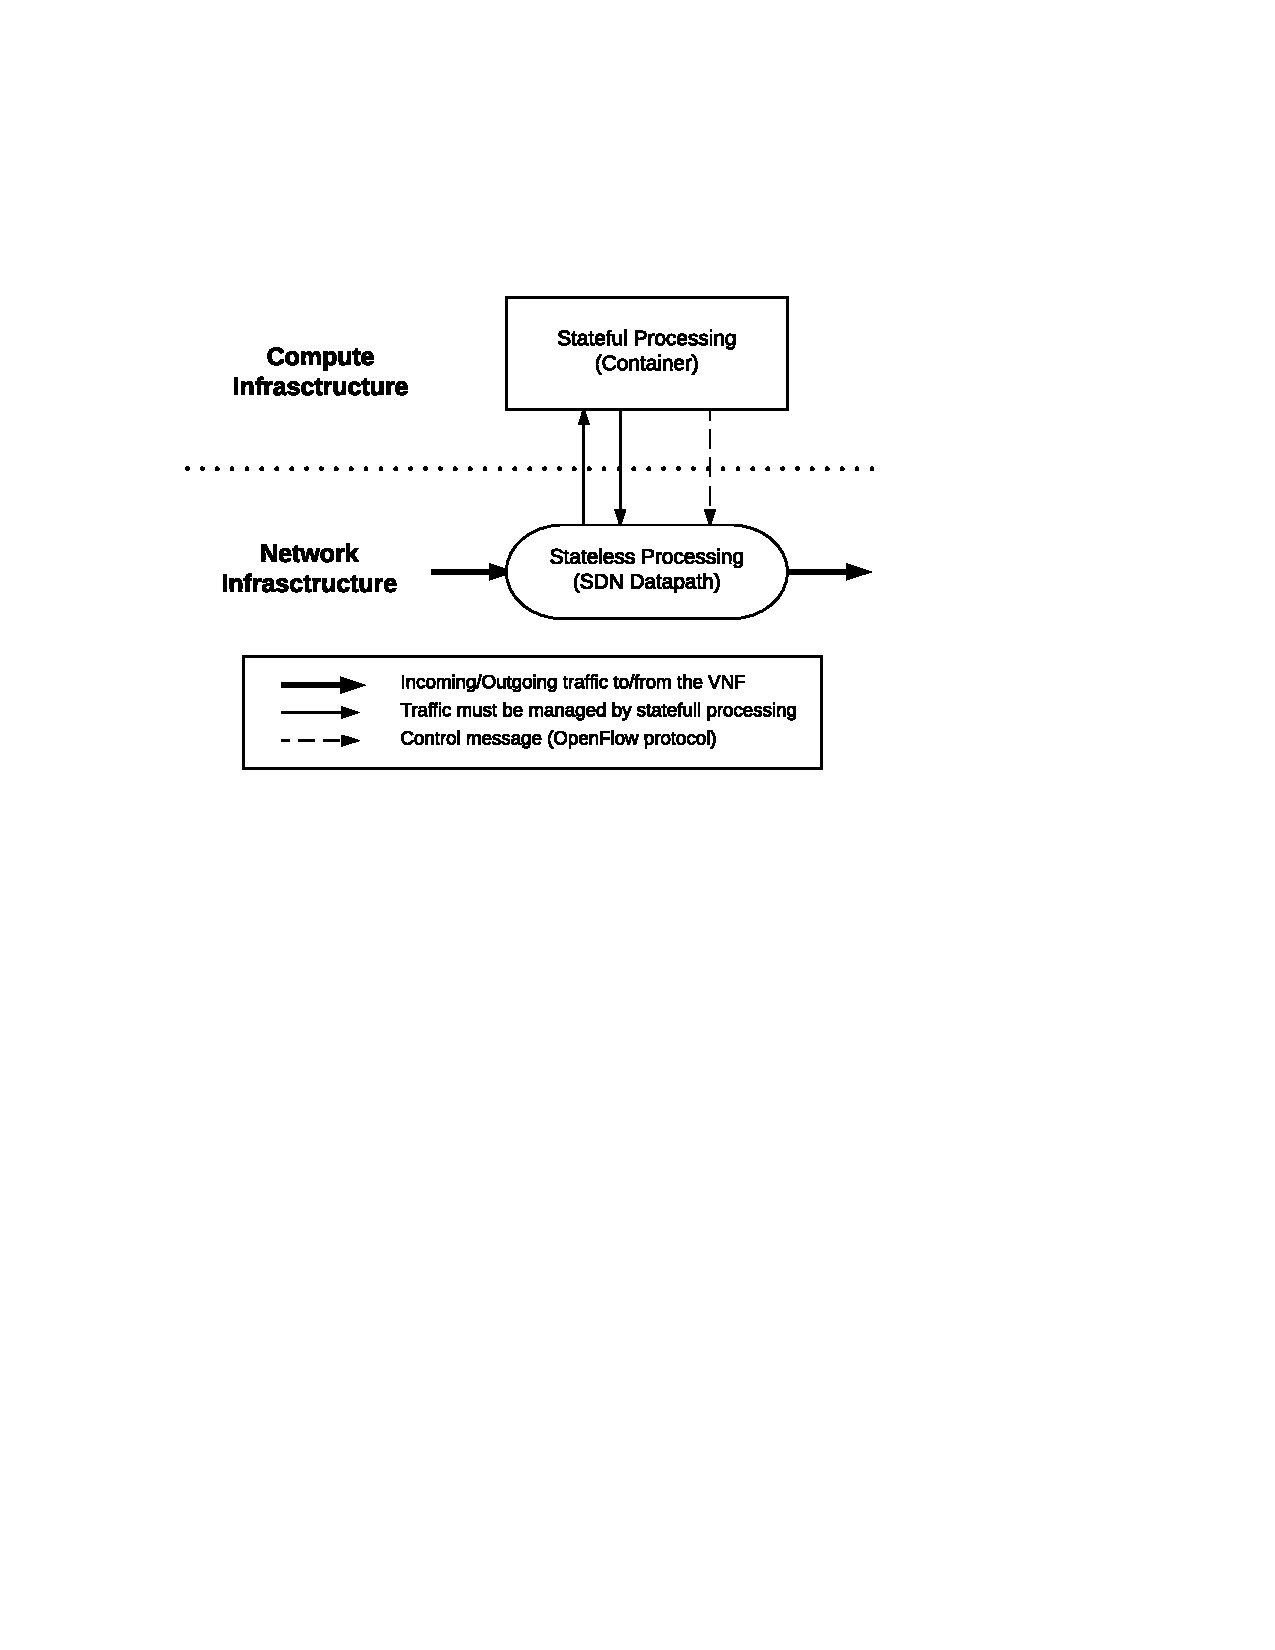
\includegraphics[width=\textwidth]{./fig/desc_nfv_overview.pdf}
\caption{Overview of network functions.}
\label{fig:desc_nfv_overview}
\end{figure}

\begin{figure*}[!t]
\centering
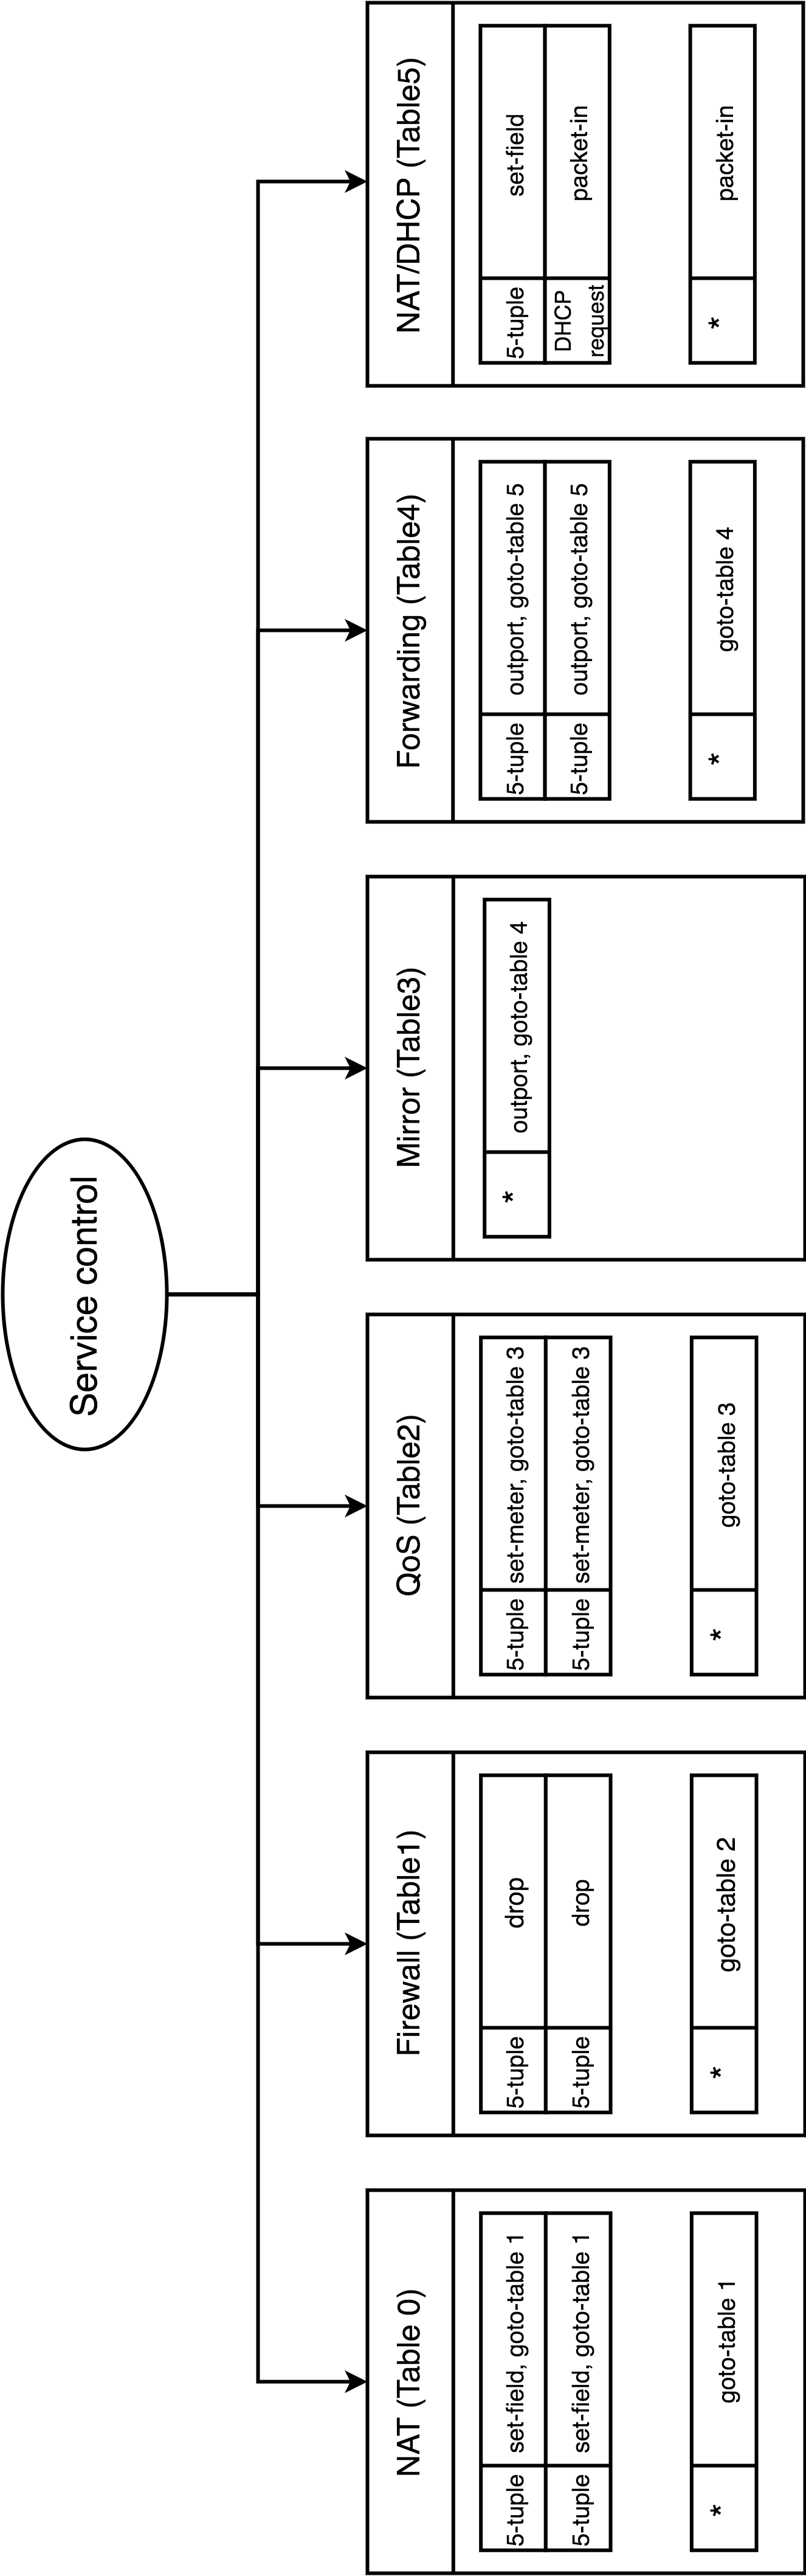
\includegraphics[width=\textwidth]{./fig/mft_table_overview}
\caption{Flow table order of vCPE service.}
\label{fig:mft_table_overview}
\end{figure*}

\section{Multiple Flow Table Strategy} \label{sec:multi_flow_table_strategy}
In section \ref{sec:desc_nfv_overview}, we introduce the vCPE service design architecture. The network functions are managed through cooperation between the SDN controller on the cloud and SDN switch at the local network gateway. The controller transforms the network functions into a series of OpenFlow rule requests and sends it to the SDN switch. Following the orders from the controller, the SDN switch inserts the rules into its flow tables, examines the incoming packets against the flow entry match fields, and executes the actions in matching rules. The flow table \cite{sdn-ft} defines all matching and corresponding processing, thus playing an important role in the executive network function.

We found that a single flow table restricts the implementation of our network functions. In \cite{multiple-flow-table}, two conditions under which a single flow table is too restrictive were reported. The first is a condition where a single packet must perform independent actions based on matching with different fields. The second is a condition where the packet requires two-stage processing. To satisfy both conditions, we implemented the network functions by using a multiple flow table strategy.

Before we discuss about the multiple flow table strategy, we introduce the pipeline of OpenFlow flow table first \cite{openflow-spec}. The processing of each packet always starts at the first flow table. When being processed by a flow table, the packet is matched the flow entries of the flow table and adds corresponding action to the instruction set. The packet can executes the instrcution set immediately, or execute after finishing the journey in switch. A flow entry can direct a packet to next table by go-to action. In our multiple flow table management model, we set the ``go to next table'' action as the table-miss action. Therefore, the packet is processed table-by-table in a certain sequence.

In a multiple flow table strategy, it is most important to determine which flow table the rules should be inserted into. We used the network function as a demarcation, that is, SDN applications responsible for specific network functions inserted rules into one specific flow table to enable us to focus on the design of the network function itself. However, the order of the flow table and the sequence of the network functions become crucial. This can be addressed by considering the type of match and action in the rules generated by the network function.

The network functions of vCPE services are the firewall service, NAT, DHCP, forwarding, and QoS. The order of each function was determined as shown in Fig. \ref{fig:mft_table_overview} (note that the flow tables are counted from zero). Each packet In the following sections, we introduce the method of implementing these network functions, the type of rules to be inserted into the SDN switch, and the effect of these rules on deciding the order of the flow tables.


\section{Service Control} \label{sec:service_control}
Service control is used to enable or disable services. To enable a service, the table-miss rule should be modified. A packet-in rule is always placed in the flow table of the last active service as a table miss in case there is no corresponding rule. To enable the service chain, the rules of each service except the last service contain an additional action, ``go to next flow table'', which enables the packets to continue to pass through all active services.

To disable a service, we must not only modify the table-miss rule but also add an enforce rule. Each enforce rule has maximum priority with the action, ``go to next flow table''. It indicates that packets still pass through the disabled service’s table, but ignore other rules and proceed to the next flow table.

\section{Network functions} \label{sec:setwork_functions}

\subsection{Firewall}
The firewall service can dynamically block traffic and prevent the packets from causing a packet-in event.
On the dashboard, we can specify the blocking policies. There are three kinds of policies:
\begin{enumerate}[leftmargin=4em]
  \item block any traffic from a source IP or destination IP address;
  \item block traffic based on known layer 4 protocols, such as SSH and HTTP;
  \item block traffic to customize layer 4 ports of a host.
\end{enumerate}

For different policies, the controller applies corresponding rules to the SDN switch. After the policies are set, the blocking rules are immediately installed. Subsequently, any traffic that satisfies the blocking criteria is dropped. Normal traffic is unaffected.

As shown in Table \ref{table:fw}, all the actions of flow entries are dropped. The first rule illustrates that SSH connection with the source IP address 192.168.2.1 is blocked. The second rule indicates that the flow entry blocks the Telnet protocol.

In our multiple flow table model, the firewall service is located in flow table 1 because once packets are detected by the blocking rules, they do not need to be applied to any other services. The packets that satisfy the blocking rules are immediately dropped, and their journey in the flow table ends. The other unblocked packets pass all blocking rules and finally satisfy the table-miss rule, which allows the packets to proceed to the next flow table. The action of the firewall is different from those of other services, because in other services, irrespective of the actions taken with the packets, the packets must proceed to the next flow table.

% firewall example table
\begin{table*}[!t]
\caption{Firewall rules in Flow Entry}
\label{table:fw}
\centering
\begin{threeparttable}
\begin{tabular}{|l|l|l|l|l|l|}
\hline
IP proto & IP src      & IP dst       & L4 sport & L4 dport & action \\ \hline
TCP      & 192.168.2.1 & *            & *        & 22       & drop   \\ \hline
TCP      & *           & *            & *        & 23       & drop   \\ \hline
\end{tabular}
  \begin{tablenotes}
    \item[] Symbol * represents wildcard (matches any value).
  \end{tablenotes}
\end{threeparttable}
\end{table*}
